% Algebra 2 Lesson 4-3 fast-track packet: Multiplying and Dividing Rational Expressions
% (enVision A2 2024 TE, Example 2 and Example 5 only; fast-lesson draft 2026-10-30, PLC has not met on this lesson)
% Quiz map (TE "4-3 Lesson Quiz"): items 1-2 simplify (Example 2); item 3 multiply (Example 3, cut;
% rehearsed by Example 5 step 1 and the sign move of Example 2); items 4-5 divide (Example 5).
% Shared preamble for the "fast" (hacked-down) Algebra 2 lesson packets, Oct 2026.
% Each packet: % Shared preamble for the "fast" (hacked-down) Algebra 2 lesson packets, Oct 2026.
% Each packet: % Shared preamble for the "fast" (hacked-down) Algebra 2 lesson packets, Oct 2026.
% Each packet: \input{fast-packet-template} then \begin{document} ... \end{document}.
\documentclass[12pt]{article}
\usepackage[margin=0.7in]{geometry}
\usepackage{amsmath,amssymb}
\usepackage{booktabs,tabularx,array}
\usepackage{enumitem}
\usepackage[T1]{fontenc}
\usepackage[utf8]{inputenc}
\usepackage{lmodern}
\usepackage{tikz}
\usepackage{pgfplots}
\pgfplotsset{compat=1.18}
\usepackage{xcolor}
\setlist{nosep,leftmargin=1.4em}
\setlength{\parindent}{0pt}
\setlength{\parskip}{6pt}
\renewcommand{\arraystretch}{1.35}
\newcolumntype{Y}{>{\raggedright\arraybackslash}X}
\pagestyle{empty}

% blanks and workspace
\newcommand{\blank}[1][2.6cm]{\rule[-2pt]{#1}{0.5pt}}
\newcommand{\lines}[1][1]{\par\vspace{2pt}\foreach \i in {1,...,#1}{\rule{0pt}{22pt}\rule{\linewidth}{0.4pt}\par}}
\newcommand{\wspart}[2]{\vspace{4pt}{\large\bfseries #1: #2}\par\vspace{-6pt}\rule{\textwidth}{0.4pt}\par}

% header: \packethead{Lesson 1-3}{Piecewise-Defined Functions}
\newcommand{\packethead}[2]{%
{\LARGE\bfseries #2}\hfill Name \blank[5cm]\\[2pt]
Algebra 2 \quad #1 (fast track) \hfill Date \blank[2.5cm] \quad Period \blank[1.2cm]\par\vspace{2pt}}

% boxed goals: \goals{learning goal}{language goal}
\newcommand{\goals}[2]{%
\fbox{\parbox{\dimexpr\textwidth-2\fboxsep-2\fboxrule}{%
\textbf{Learning goal:} #1\\[2pt]
\textbf{Language goal:} #2}}\par}

% quiz target box: \quiztarget{text}
\newcommand{\quiztarget}[1]{%
\vspace{4pt}\colorbox{gray!12}{\parbox{\dimexpr\textwidth-2\fboxsep}{\textbf{On the quiz:} #1}}\par}

% IXL table row helper: code & skill & which quiz question it feeds
\newcommand{\ixlrow}[3]{\texttt{#1} & #2 & #3 \\}

% one grid style for every graph; override xmin/xmax/... per plot
\pgfplotsset{sheetgrid/.style={
  axis lines=middle, grid=both, grid style={gray!45},
  xmin=-10.5, xmax=10.5, ymin=-10.5, ymax=10.5,
  xtick={-10,-8,...,10}, ytick={-10,-8,...,10},
  x=0.28cm, y=0.28cm,
  ticklabel style={font=\scriptsize, fill=white, inner sep=1pt},
  xlabel={$x$}, ylabel={$y$},
  axis line style={thick}, clip=true}}
% unit grid for small windows
\pgfplotsset{unitgrid/.style={sheetgrid,
  xmin=-5.5, xmax=5.5, ymin=-5.5, ymax=5.5,
  xtick={-5,...,5}, ytick={-5,...,5}, x=0.5cm, y=0.5cm}}
% open and closed endpoints
\tikzset{closed/.style={circle, fill, inner sep=1.6pt},
         open/.style={circle, draw, fill=white, inner sep=1.4pt}}
 then \begin{document} ... \end{document}.
\documentclass[12pt]{article}
\usepackage[margin=0.7in]{geometry}
\usepackage{amsmath,amssymb}
\usepackage{booktabs,tabularx,array}
\usepackage{enumitem}
\usepackage[T1]{fontenc}
\usepackage[utf8]{inputenc}
\usepackage{lmodern}
\usepackage{tikz}
\usepackage{pgfplots}
\pgfplotsset{compat=1.18}
\usepackage{xcolor}
\setlist{nosep,leftmargin=1.4em}
\setlength{\parindent}{0pt}
\setlength{\parskip}{6pt}
\renewcommand{\arraystretch}{1.35}
\newcolumntype{Y}{>{\raggedright\arraybackslash}X}
\pagestyle{empty}

% blanks and workspace
\newcommand{\blank}[1][2.6cm]{\rule[-2pt]{#1}{0.5pt}}
\newcommand{\lines}[1][1]{\par\vspace{2pt}\foreach \i in {1,...,#1}{\rule{0pt}{22pt}\rule{\linewidth}{0.4pt}\par}}
\newcommand{\wspart}[2]{\vspace{4pt}{\large\bfseries #1: #2}\par\vspace{-6pt}\rule{\textwidth}{0.4pt}\par}

% header: \packethead{Lesson 1-3}{Piecewise-Defined Functions}
\newcommand{\packethead}[2]{%
{\LARGE\bfseries #2}\hfill Name \blank[5cm]\\[2pt]
Algebra 2 \quad #1 (fast track) \hfill Date \blank[2.5cm] \quad Period \blank[1.2cm]\par\vspace{2pt}}

% boxed goals: \goals{learning goal}{language goal}
\newcommand{\goals}[2]{%
\fbox{\parbox{\dimexpr\textwidth-2\fboxsep-2\fboxrule}{%
\textbf{Learning goal:} #1\\[2pt]
\textbf{Language goal:} #2}}\par}

% quiz target box: \quiztarget{text}
\newcommand{\quiztarget}[1]{%
\vspace{4pt}\colorbox{gray!12}{\parbox{\dimexpr\textwidth-2\fboxsep}{\textbf{On the quiz:} #1}}\par}

% IXL table row helper: code & skill & which quiz question it feeds
\newcommand{\ixlrow}[3]{\texttt{#1} & #2 & #3 \\}

% one grid style for every graph; override xmin/xmax/... per plot
\pgfplotsset{sheetgrid/.style={
  axis lines=middle, grid=both, grid style={gray!45},
  xmin=-10.5, xmax=10.5, ymin=-10.5, ymax=10.5,
  xtick={-10,-8,...,10}, ytick={-10,-8,...,10},
  x=0.28cm, y=0.28cm,
  ticklabel style={font=\scriptsize, fill=white, inner sep=1pt},
  xlabel={$x$}, ylabel={$y$},
  axis line style={thick}, clip=true}}
% unit grid for small windows
\pgfplotsset{unitgrid/.style={sheetgrid,
  xmin=-5.5, xmax=5.5, ymin=-5.5, ymax=5.5,
  xtick={-5,...,5}, ytick={-5,...,5}, x=0.5cm, y=0.5cm}}
% open and closed endpoints
\tikzset{closed/.style={circle, fill, inner sep=1.6pt},
         open/.style={circle, draw, fill=white, inner sep=1.4pt}}
 then \begin{document} ... \end{document}.
\documentclass[12pt]{article}
\usepackage[margin=0.7in]{geometry}
\usepackage{amsmath,amssymb}
\usepackage{booktabs,tabularx,array}
\usepackage{enumitem}
\usepackage[T1]{fontenc}
\usepackage[utf8]{inputenc}
\usepackage{lmodern}
\usepackage{tikz}
\usepackage{pgfplots}
\pgfplotsset{compat=1.18}
\usepackage{xcolor}
\setlist{nosep,leftmargin=1.4em}
\setlength{\parindent}{0pt}
\setlength{\parskip}{6pt}
\renewcommand{\arraystretch}{1.35}
\newcolumntype{Y}{>{\raggedright\arraybackslash}X}
\pagestyle{empty}

% blanks and workspace
\newcommand{\blank}[1][2.6cm]{\rule[-2pt]{#1}{0.5pt}}
\newcommand{\lines}[1][1]{\par\vspace{2pt}\foreach \i in {1,...,#1}{\rule{0pt}{22pt}\rule{\linewidth}{0.4pt}\par}}
\newcommand{\wspart}[2]{\vspace{4pt}{\large\bfseries #1: #2}\par\vspace{-6pt}\rule{\textwidth}{0.4pt}\par}

% header: \packethead{Lesson 1-3}{Piecewise-Defined Functions}
\newcommand{\packethead}[2]{%
{\LARGE\bfseries #2}\hfill Name \blank[5cm]\\[2pt]
Algebra 2 \quad #1 (fast track) \hfill Date \blank[2.5cm] \quad Period \blank[1.2cm]\par\vspace{2pt}}

% boxed goals: \goals{learning goal}{language goal}
\newcommand{\goals}[2]{%
\fbox{\parbox{\dimexpr\textwidth-2\fboxsep-2\fboxrule}{%
\textbf{Learning goal:} #1\\[2pt]
\textbf{Language goal:} #2}}\par}

% quiz target box: \quiztarget{text}
\newcommand{\quiztarget}[1]{%
\vspace{4pt}\colorbox{gray!12}{\parbox{\dimexpr\textwidth-2\fboxsep}{\textbf{On the quiz:} #1}}\par}

% IXL table row helper: code & skill & which quiz question it feeds
\newcommand{\ixlrow}[3]{\texttt{#1} & #2 & #3 \\}

% one grid style for every graph; override xmin/xmax/... per plot
\pgfplotsset{sheetgrid/.style={
  axis lines=middle, grid=both, grid style={gray!45},
  xmin=-10.5, xmax=10.5, ymin=-10.5, ymax=10.5,
  xtick={-10,-8,...,10}, ytick={-10,-8,...,10},
  x=0.28cm, y=0.28cm,
  ticklabel style={font=\scriptsize, fill=white, inner sep=1pt},
  xlabel={$x$}, ylabel={$y$},
  axis line style={thick}, clip=true}}
% unit grid for small windows
\pgfplotsset{unitgrid/.style={sheetgrid,
  xmin=-5.5, xmax=5.5, ymin=-5.5, ymax=5.5,
  xtick={-5,...,5}, ytick={-5,...,5}, x=0.5cm, y=0.5cm}}
% open and closed endpoints
\tikzset{closed/.style={circle, fill, inner sep=1.6pt},
         open/.style={circle, draw, fill=white, inner sep=1.4pt}}

% local header: the TE title is too long to share a line with Name (template macro unchanged)
\renewcommand{\packethead}[2]{%
{\LARGE\bfseries #2}\par\vspace{4pt}
Algebra 2 \quad #1 (fast track) \hfill Name \blank[4cm] \quad Date \blank[2cm] \quad Period \blank[0.9cm]\par\vspace{2pt}}
\begin{document}

\packethead{Lesson 4-3}{Multiplying and Dividing Rational Expressions}
\goals{I can simplify a rational expression and find the product and the quotient of rational expressions, and state the domain.}{I can explain how I simplified a rational expression using the words factor, common factor, reciprocal, domain and simplified form.}
\vspace{-4pt}{\footnotesize Spanish: \emph{expresión racional} (rational expression), \emph{máximo factor común} (greatest common factor).}

\vspace{-4pt}\quiztarget{(2) graded: simplify and state the domain. Factor, take the domain from the \emph{original} denominator, divide out common factors (Example 2). (4) graded: divide. Multiply by the reciprocal of the divisor, then factor and divide out (Example 5). (5) bonus: width $=$ area $\div$ length (the Practice after Try It 5). (1) simplify and (3) multiply: full Savvas quiz only.}

\wspart{Example 2}{Simplify a Rational Expression}
What is the simplified form of the rational expression $\dfrac{4-x^2}{x^2+3x-10}$? What is the domain for which the identity between the two expressions is valid? The \textbf{simplified form} has no common factors, other than 1, in the numerator and the denominator.

\begin{minipage}[t]{0.58\textwidth}
\vspace{-8pt}
\begin{align*}
\frac{4-x^2}{x^2+3x-10}&=\frac{(2-x)(2+x)}{(x-2)(x+5)} && \textbf{factor}\\
&=\frac{-(x-2)(x+2)}{(x-2)(x+5)} && 2-x=-1(x-2)\\
&=-\frac{x-2}{x-2}\cdot\frac{x+2}{x+5} && \text{\small\textbf{common factor}}\\
&=-\frac{x+2}{x+5} && \text{\small divides to 1}
\end{align*}
\textbf{Domain} (from the \emph{original} denominator): $(x-2)(x+5)=0$ when $x=2$ or $x=-5$, so exclude both.
\end{minipage}\hfill
\begin{minipage}[t]{0.38\textwidth}
\vspace{0pt}
\fbox{\parbox{\dimexpr\linewidth-2\fboxsep-2\fboxrule}{%
\textbf{Simplified form:}\\[2pt]
\centerline{$-\dfrac{x+2}{x+5}$ \ for $x\neq 2$ or $-5$}}}

\vspace{4pt}
\textbf{Check} $x=0$: original $\dfrac{4-0}{0+0-10}=-\dfrac{2}{5}$; simplified $-\dfrac{0+2}{0+5}=-\dfrac{2}{5}$ \checkmark

\vspace{4pt}
{\small\textbf{Watch out:} only \emph{factors} divide out, never terms. You cannot cross out the $x^2$ terms.}
\end{minipage}

\textbf{Say it:} I \blank[1.8cm] the top and the bottom. The common factor \blank[1.8cm] divides to 1. The domain leaves out $x=$\,\blank[1cm] and $x=$\,\blank[1cm] because they make the \blank[2.8cm] equal zero.

\wspart{Try It 2}{Simplify each expression and state the domain}
\begin{minipage}[t]{0.48\textwidth}
\vspace{0pt}
\textbf{a.} $\dfrac{x^2+2x+1}{x^3-2x^2-3x}$
\lines[3]
Simplified: \blank[2cm] \ Domain: $x\neq$\,\blank[1.5cm]
\end{minipage}\hfill
\begin{minipage}[t]{0.48\textwidth}
\vspace{0pt}
\textbf{b.} $\dfrac{x^3+4x^2-x-4}{x^2+3x-4}$

{\small Hint: factor the numerator by grouping.}
\lines[3]
Simplified: \blank[2cm] \ Domain: $x\neq$\,\blank[1.5cm]
\end{minipage}

\newpage
\wspart{Example 5}{Divide Rational Expressions}
What is the quotient of $\dfrac{x^3+3x^2+3x+1}{1-x^2}$ and $\dfrac{x^2+5x+4}{x^2+3x-4}$?

\textbf{The idea:} divide fractions the way you always have. Multiply by the \textbf{reciprocal} of the divisor (flip the second fraction), then it is a multiplication problem.

\begin{enumerate}[label=\textbf{\arabic*.}, itemsep=4pt]
\item Multiply by the \textbf{reciprocal} of the divisor.
\[\frac{x^3+3x^2+3x+1}{1-x^2}\div\frac{x^2+5x+4}{x^2+3x-4}=\frac{x^3+3x^2+3x+1}{1-x^2}\cdot\frac{x^2+3x-4}{x^2+5x+4}\]
\item \textbf{Factor} every polynomial.\\[2pt]
\begin{tabular}{@{}ll@{}}
$x^3+3x^2+3x+1=(x+1)(x+1)(x+1)$ & (a perfect cube: $(x+1)^3$)\\
$1-x^2=(1-x)(1+x)=-(x-1)(x+1)$ & (opposites again, like Example 2)\\
$x^2+3x-4=(x+4)(x-1)$ & $x^2+5x+4=(x+1)(x+4)$
\end{tabular}
\item \textbf{Domain:} leave out every $x$ that makes a denominator zero, \emph{including the divisor's numerator}, because it moved to the bottom.\\
$1-x^2=0$: $x=\pm1$; \quad $x^2+3x-4=0$: $x=-4,\,1$; \quad $x^2+5x+4=0$: $x=-1,\,-4$. \quad So $x\neq-4,\,-1,\,1$.
\item Divide out the \textbf{common factors}.
\[=\frac{(x+1)(x+1)(x+1)(x+4)(x-1)}{-(x-1)(x+1)(x+1)(x+4)}
=\frac{x+1}{-1}\cdot\frac{x+1}{x+1}\cdot\frac{x+1}{x+1}\cdot\frac{x-1}{x-1}\cdot\frac{x+4}{x+4}\]
\end{enumerate}

\begin{minipage}[t]{0.48\textwidth}
\vspace{0pt}
\fbox{\parbox{\dimexpr\linewidth-2\fboxsep-2\fboxrule}{%
\textbf{The quotient is} $-(x+1)$, \ $x\neq-4,\,-1,\text{ or }1$.}}
\end{minipage}\hfill
\begin{minipage}[t]{0.48\textwidth}
\vspace{0pt}
\textbf{Check} with $x=0$: $\dfrac{1}{1}\div\dfrac{4}{-4}=1\div(-1)=-1$, and $-(0+1)=-1$ \checkmark
\end{minipage}

\vspace{4pt}
\textbf{Say it:} To divide, I multiplied by the \blank[2.4cm] of the divisor. Then I \blank[2cm] every polynomial and divided out the \blank[3cm]. The domain leaves out $x=$\,\blank[2.6cm] because \lines[1]

\wspart{Try It 5}{Find the simplified quotient and the domain of each expression}
\begin{minipage}[t]{0.48\textwidth}
\vspace{0pt}
\textbf{a.} $\dfrac{1}{x^2+9x}\div\left(\dfrac{6-x}{3x^2-18x}\right)$
\lines[5]
Quotient: \blank[3.5cm]\\[4pt]
Domain: all $x$ except \blank[2.6cm]
\end{minipage}\hfill
\begin{minipage}[t]{0.48\textwidth}
\vspace{0pt}
\textbf{b.} $\dfrac{2x^2-12x}{x+5}\div\left(\dfrac{x-6}{x+5}\right)$
\lines[5]
Quotient: \blank[3.5cm]\\[4pt]
Domain: all $x$ except \blank[2.6cm]
\end{minipage}

\newpage
% R5 Practice: rehearses Lesson Quiz item 5 (rectangle: width = area / length), which no Try It covers.
% TE Practice & Problem Solving 37 (Example 6, DOK 2), verbatim: same structure (one dimension = area / other dimension), different shape and numbers.
\wspart{Practice}{Area divided by one dimension (Practice 37)}
\begin{minipage}[t]{0.56\textwidth}
\vspace{0pt}
A parallelogram with an area of $\dfrac{3x+12}{10x+25}$ square units has a height shown. Find the length of the base of the parallelogram.

\vspace{4pt}
\textbf{a.} Area $=$ base $\times$ height, so base $=$ area $\div$ \blank[1.6cm].

\textbf{b.} Multiply by the reciprocal, factor, and divide out the common factors.
\lines[3]
\textbf{c.} Base $=$ \blank[2.5cm] units.
\end{minipage}\hfill
\begin{minipage}[t]{0.40\textwidth}
\vspace{6pt}
\begin{center}
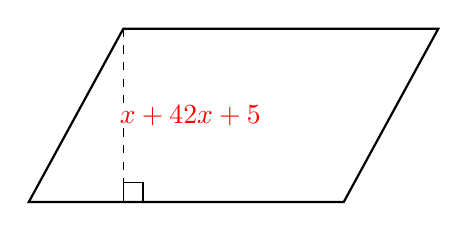
\begin{tikzpicture}[scale=1]
\draw[thick] (0,0) -- (4,0) -- (5.2,2.2) -- (1.2,2.2) -- cycle;
\draw[dashed] (1.2,2.2) -- (1.2,0);
\draw (1.2,0) rectangle (1.45,0.25);
\node[red, fill=white, inner sep=1pt] at (2.05,1.1) {$\dfrac{x+4}{2x+5}$};
\end{tikzpicture}
\end{center}
\end{minipage}

\wspart{IXL}{Practice for the quiz}
Go to IXL, Algebra 2. Type the code in the search box. Do the starred skills first.

\vspace{2pt}
\begin{tabularx}{\textwidth}{l l Y}
\toprule
\textbf{Code} & \textbf{Skill} & \textbf{Feeds} \\
\midrule
\ixlrow{37N $\bigstar$}{Simplify rational expressions}{Quiz 2; Quiz 1 (full Savvas quiz only)}
\ixlrow{79Q $\bigstar$}{Domain of rational functions}{Quiz 2: the domain (Example 2, step 2)}
\ixlrow{MG2 $\bigstar$}{Multiply and divide rational expressions}{Quiz 4, 5; Quiz 3 (full Savvas quiz only)}
\ixlrow{UB5}{Factor quadratics}{Warm-up: every problem starts by factoring}
\ixlrow{QKF}{Factor using a quadratic pattern}{Warm-up: $4-x^2$, $9-x^2$, $x^2+6x+9$}
\bottomrule
\end{tabularx}

\textbf{SmartScore 70 or above on each starred ($\bigstar$) skill replaces your quiz score.}

% R3: the lesson's only DOK 3 (Practice & Problem Solving 13, Higher Order Thinking, Example 5).
\wspart{Exit question}{Practice 13 (DOK 3)}
\fbox{\parbox{\dimexpr\textwidth-2\fboxsep-2\fboxrule}{%
Why are rational expressions closed under multiplication and division?

\vspace{4pt}
Start from two rational expressions $\dfrac{a}{b}$ and $\dfrac{c}{d}$, where $a$, $b$, $c$, $d$ are polynomials and $b,d\neq0$.

\vspace{4pt}
$\dfrac{a}{b}\cdot\dfrac{c}{d}=$\,\blank[2.5cm]. \ The top and the bottom are both \blank[3cm], so the product is a \blank[3cm].

\vspace{6pt}
$\dfrac{a}{b}\div\dfrac{c}{d}=\dfrac{a}{b}\cdot$\,\blank[1.5cm] because dividing means multiplying by the \blank[2.5cm]. So the quotient is also a \blank[3.5cm] (as long as $c\neq0$).\par\vspace{4pt}}}

\textbf{Before the quiz, finish this sentence.} To simplify a product or quotient, I first \blank[2cm] every polynomial. The \blank[2cm] leaves out every $x$ that makes an original denominator zero or, in a quotient, the divisor's numerator zero. Last I divide out each \blank[3cm].

\end{document}
